\documentclass[11pt, oneside]{article}   	% use "amsart" instead of "article" for AMSLaTeX format
\usepackage{geometry}                		% See geometry.pdf to learn the layout options. There are lots.
\geometry{letterpaper}                   		% ... or a4paper or a5paper or ... 
%\geometry{landscape}                		% Activate for rotated page geometry
\usepackage[parfill]{parskip}    		% Activate to begin paragraphs with an empty line rather than an indent
\usepackage{graphicx}				% Use pdf, png, jpg, or eps§ with pdflatex; use eps in DVI mode
								% TeX will automatically convert eps --> pdf in pdflatex		
								
\usepackage{listings}				% Source code
\usepackage{xcolor}					% colour (source code for instance)
\definecolor{grey}{rgb}{0.1,0.1,0.1}
\definecolor{darkblue}{rgb}{0.0,0.0,0.6}
\definecolor{cyan}{rgb}{0.0,0.6,0.6}

\usepackage{amssymb}
\usepackage{cite}
\usepackage{hyperref}				% Hyperlinks
\usepackage[nottoc,numbib]{tocbibind}	% 'References' in TOC

\graphicspath{{img/}}					% Relative path where the images are stored. 

\title{Instructions for \\ Web Audio Evaluation Tool}
\author{Nicholas Jillings, Brecht De Man and David Moffat}
\date{7 December 2015}							% Activate to display a given date or no date

\begin{document}
\maketitle

These instructions are about use of the Web Audio Evaluation Tool on Windows and Mac OS X platforms. 

We request that you acknowledge the authors and cite our work when using it \cite{waet}, see also CITING.txt. 

The tool is available in its entirety including source code on \url{https://code.soundsoftware.ac.uk/projects/webaudioevaluationtool/}, under the GNU General Public License v3.0 (\url{http://choosealicense.com/licenses/gpl-3.0/}), see also LICENSE.txt. 

% TO DO: Linux (Android, iOS)

\tableofcontents

\clearpage

\section{Installation}
	Download the folder (\url{https://code.soundsoftware.ac.uk/hg/webaudioevaluationtool/archive/tip.zip}) and unzip in a location of your choice, or pull the source code from \url{https://code.soundsoftware.ac.uk/hg/webaudioevaluationtool} (Mercurial). 
	
	\subsection{Contents}
		The folder should contain the following elements: \\
		
		\textbf{Main folder:} 
			\begin{itemize}
	            	\item \texttt{analyse.html}: analysis and diagnostics of a set of result XML files
	            	\item \texttt{core.css, graphics.css, structure.css}: core style files (edit to change appearance)
	            	\item \texttt{CITING.txt, LICENSE.txt, README.txt}: text files with, respectively, the citation which we ask to include in any work where this tool or any portion thereof is used, modified or otherwise; the license under which the software is shared; and a general readme file referring to these instructions.
	            	\item \texttt{core.js}: JavaScript file with core functionality
	            	\item \texttt{index.html}: webpage where interface should appear (includes link to test configuration XML)
	            	\item \texttt{jquery-2.1.4.js}: jQuery JavaScript Library
	            	\item \texttt{loudness.js}: Allows for automatic calculation of loudness of Web Audio API Buffer objects, return gain values to correct for a target loudness or match loudness between multiple objects
	            	\item \texttt{pythonServer.py}: webserver for running tests locally
	            	\item \texttt{pythonServer-legacy.py}: webserver with limited functionality (no automatic storing of output XML files)
	            	\item \texttt{save.php}: PHP script to store result XML files to web server\\
			\end{itemize}
	     \textbf{Documentation (./docs/)}
	         \begin{itemize}
	         		\item \href{http://c4dm.eecs.qmul.ac.uk/dmrn/events/dmrnp10/#posters}{DMRN+10}: PDF and \LaTeX source of poster for 10\textsuperscript{th} Digital Music Research Network One-Day workshop (``soft launch'')
	         		\item Instructions: PDF and \LaTeX source of these instructions
	            	\item Project Specification Document (\LaTeX/PDF)
	            	\item Results Specification Document (\LaTeX/PDF)
	            	\item SMC15: PDF and \LaTeX  source of 12th Sound and Music Computing Conference paper \cite{waet}
	            	\item WAC2016: PDF and \LaTeX  source of 2nd Web Audio Conference paper\\
			\end{itemize}
         \textbf{Example project (./example\_eval/)}
            	\begin{itemize}
            		\item An example of what the set up XML should look like, with example audio files 0.wav-10.wav which are short recordings at 44.1kHz, 16bit of a woman saying the corresponding number (useful for testing randomisation and general familiarisation with the interface).\\ 
            	\end{itemize}
          \textbf{Interface files (./interfaces/}
              \begin{itemize}
                  \item Each interface class has a JavaScript file and an optional CSS style file. These are loaded as needed.
              \end{itemize}

          \textbf{Output files (./saves/)}
            	\begin{itemize}
            		\item The output XML files of tests will be stored here by default by the \texttt{pythonServer.py} script.\\ 
            	\end{itemize}
          \textbf{Auxiliary scripts (./scripts/)}
            	\begin{itemize}
            		\item Helpful Python scripts for extraction and visualisation of data.\\ 
            	\end{itemize}
          \textbf{Test creation tool (./test\_create/)}
            	\begin{itemize}
            		\item Webpage for easily setting up your own test without having to delve into the XML.\\ 
            	\end{itemize}
                    	
	\subsection{Compatibility}
		As Microsoft Internet Explorer doesn't support the Web Audio API\footnote{\url{http://caniuse.com/\#feat=audio-api}}, you will need another browser like Google Chrome, Safari or Firefox (all three are tested and confirmed to work). 

		Firefox does not currently support other bit depths than 8 or 16 bit for PCM wave files. In the future, this will throw a warning message to tell the user that their content is being quantised automatically. %Nick? Right? To be removed if and when actually implemented
		
		The tool is platform-independent and works in any browser that supports the Web Audio API. It does not require any specific, proprietary software. However, in case the tool is hosted locally (i.e. you are not hosting it on an actual webserver) you will need Python (2.7), which is a free programming language - see the next paragraph. 
	
\clearpage


\section{Test setup}

	\subsection{Sample rate}
		Depending on how the experiment is set up, audio is resampled automatically (the Web Audio default) or the sample rate is enforced. In the latter case, you will need to make sure that the sample rate of the system is equal to the sample rate of these audio files. For this reason, all audio files in the experiment will have to have the same sample rate. 

		Always make sure that all other digital equipment in the playback chain (clock, audio interface, digital-to-analog converter, ...) is set to this same sample rate.

		Note that upon changing the sampling rate, the browser will have to be restarted for the change to take effect. 
		
		\subsubsection{Mac OS X}
			To change the sample rate in Mac OS X, go to \textbf{Applications/Utilities/Audio MIDI Setup} or find this application with Spotlight (see Figure \ref{fig:audiomidisetup}). Then select the output of the audio interface you are using and change the `Format' to the appropriate number. Also make sure the bit depth and channel count are as desired. 
			If you are using an external audio interface, you may have to go to the preference pane of that device to change the sample rate. 

			Also make sure left and right channel gains are equal, as some applications alter this without changing it back, leading to a predominantly louder left or right channel. See Figure \ref{fig:audiomidisetup} for an example where the channel gains are different. 

			\begin{figure}[tb]
				\centering
				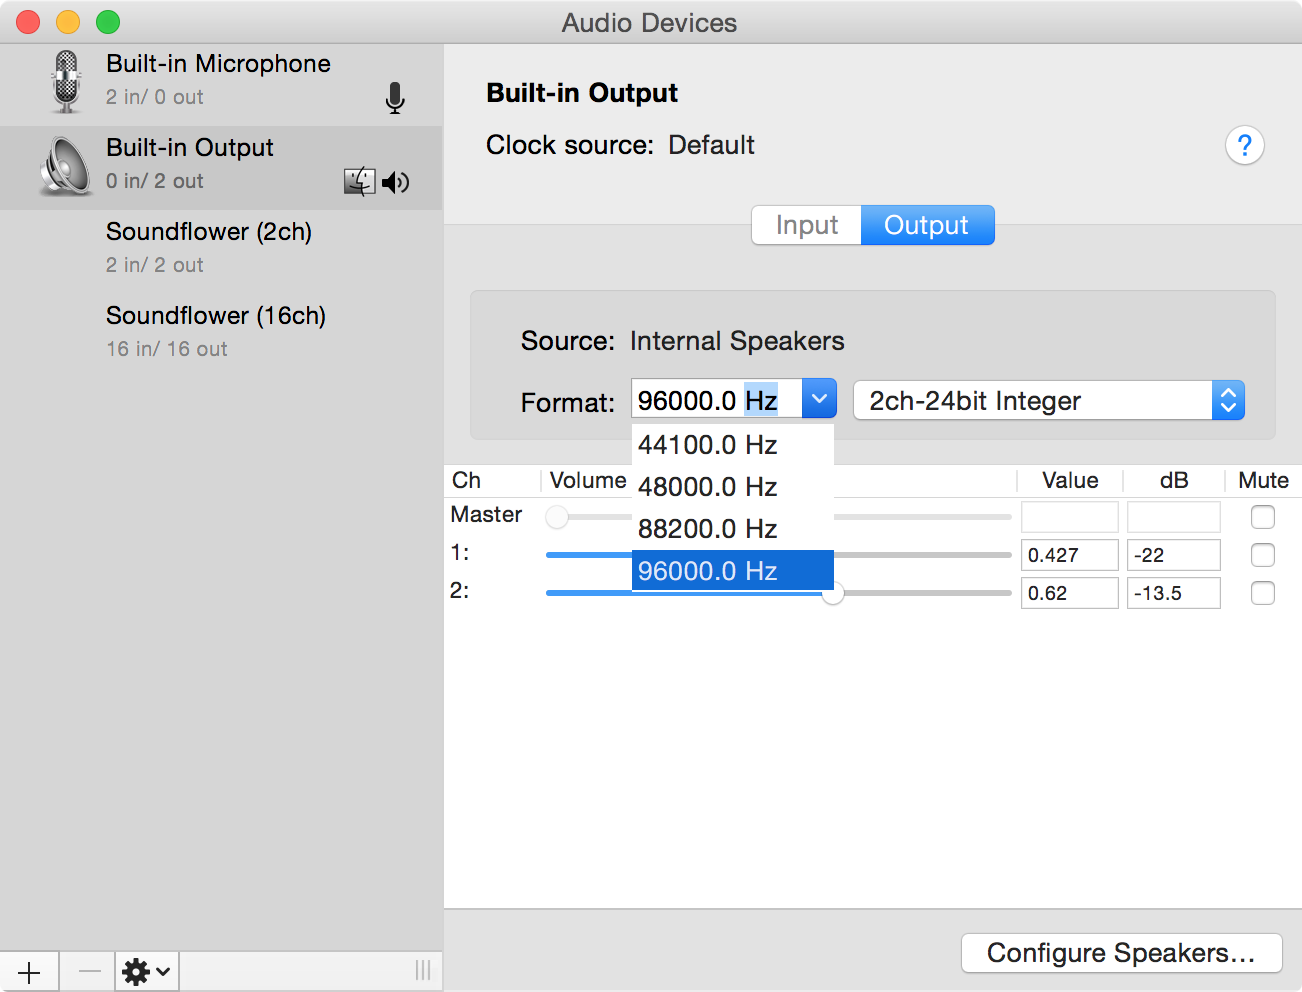
\includegraphics[width=.65\textwidth]{img/audiomidisetup.png}
				\caption{The Audio MIDI Setup window in Mac OS X}
				\label{fig:audiomidisetup}
			\end{figure}
		
		\subsubsection{Windows}
			To change the sample rate in Windows, right-click on the speaker icon in the lower-right corner of your desktop and choose `Playback devices'. Right-click the appropriate playback device and click `Properties'. Click the `Advanced' tab and verify or change the sample rate under `Default Format'.    % NEEDS CONFIRMATION
			If you are using an external audio interface, you may have to go to the preference pane of that device to change the sample rate. 

	\subsection{Local test}
		If the test is hosted locally, you will need to run the local webserver provided with this tool. 
		
		\subsubsection{Mac OS X \& Linux}

			On Mac OS X, Python comes preinstalled, as with most Unix/Linux distributions.

			Open the Terminal (find it in \textbf{Applications/Terminal} or via Spotlight), and go to the folder you downloaded. To do this, type \texttt{cd [folder]}, where \texttt{[folder]} is the folder where to find the \texttt{pythonServer.py} script you downloaded. For instance, if the location is \texttt{/Users/John/Documents/test/}, then type
			
				\texttt{cd /Users/John/Documents/test/}
				
			Then hit enter and run the Python script by typing

				\texttt{python pythonServer.py}

			and hit enter again. See also Figure \ref{fig:terminal}.
			
			\begin{figure}[htbp]
	                \begin{center}
	                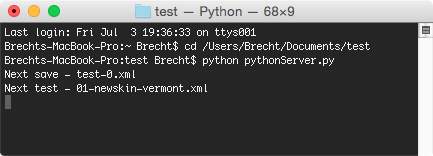
\includegraphics[width=.75\textwidth]{pythonServer.png}
	                \caption{Mac OS X: The Terminal window after going to the right folder (\texttt{cd [folder\_path]}) and running \texttt{pythonServer.py}.}
	                \label{fig:terminal}
	                \end{center}
	                \end{figure}

	        Alternatively, you can simply type \texttt{python} (follwed by a space) and drag the file into the Terminal window from Finder. % DOESN'T WORK YET
			
			You can leave this running throughout the different experiments (i.e. leave the Terminal open). Once running the terminal will report the current URL to type into your browser to initiate the test, usually this is http://localhost:8000/.

			To start the test, open the browser and type 
				
			\texttt{localhost:8000}

			and hit enter. The test should start (see Figure \ref{fig:test}). 

			To quit the server, either close the terminal window or press Ctrl+C on your keyboard to forcibly shut the server.

		\subsubsection{Windows}

			On Windows, Python 2.7 is not generally preinstalled and therefore has to be downloaded\footnote{\url{https://www.python.org/downloads/windows/}} and installed to be able to run scripts such as the local webserver, necessary if the tool is hosted locally. 
		
			Simply double click the Python script \texttt{pythonServer.py} in the folder you downloaded. 
			
			You may see a warning like the one in Figure \ref{fig:warning}. Click `Allow access'. 
			
			\begin{figure}[htbp]
            \begin{center}
            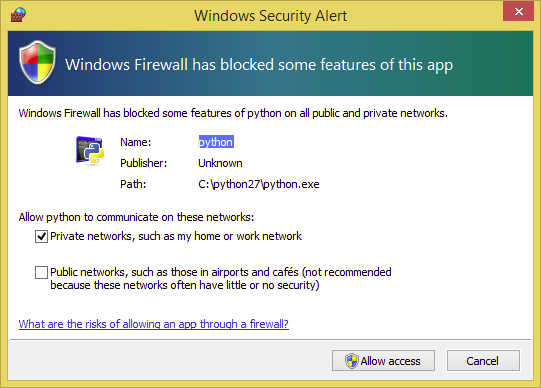
\includegraphics[width=.6\textwidth]{warning.png}
            \caption{Windows: Potential warning message when executing \texttt{pythonServer.py}.}
            \label{fig:warning}
            \end{center}
            \end{figure}
            
            The process should now start, in the Command prompt that opens - see Figure \ref{fig:python}. 
            
            \begin{figure}[htbp]
            \begin{center}
            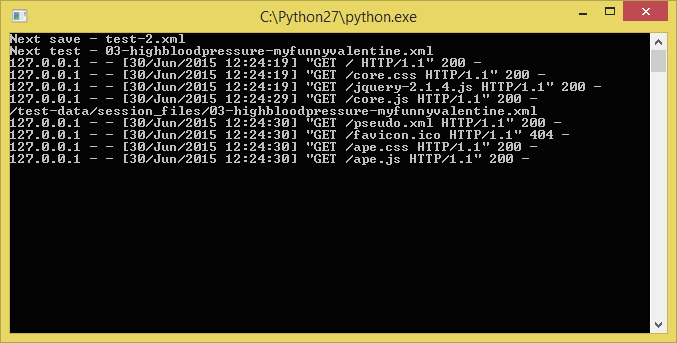
\includegraphics[width=.75\textwidth]{python.png}
            \caption{Windows: The Command Prompt after running \texttt{pythonServer.py} and opening the corresponding website.}
            \label{fig:python}
            \end{center}
            \end{figure}
            
            You can leave this running throughout the different experiments (i.e. leave the Command Prompt open). 

		    To start the test, open the browser and type 
				
			\texttt{localhost:8000}
		
			and hit enter. The test should start (see Figure \ref{fig:test}). 
		
			\begin{figure}[htb]
	        \begin{center}
	        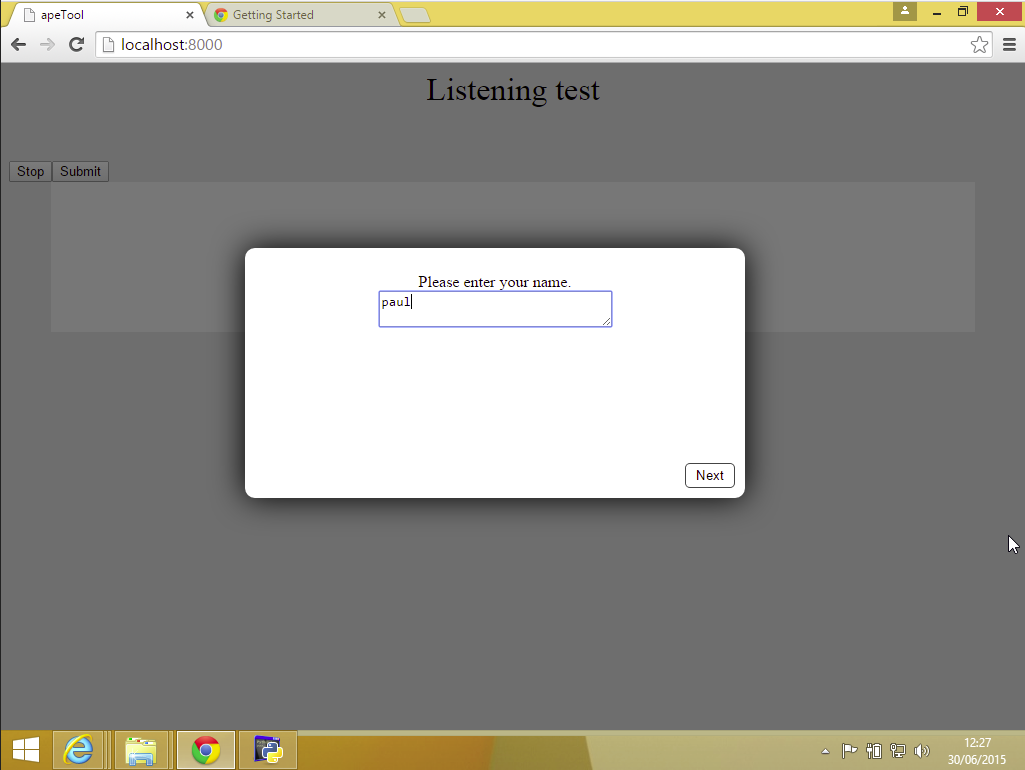
\includegraphics[width=.8\textwidth]{test.png}
	        \caption{The start of the test in Google Chrome on Windows 7.}
	        \label{fig:test}
	        \end{center}
	        \end{figure}
                    
        If at any point in the test the participant reports weird behaviour or an error of some kind, or the test needs to be interrupted, please notify the experimenter and/or refer to Section \ref{sec:troubleshooting}. 
		
		When the test is over (the subject should see a message to that effect, and click `Submit' one last time), the output XML file containing all collected data should have appeared in `saves/'. The names of these files are `test-0.xml', `test-1.xml', etc., in ascending order. The Terminal or Command prompt running the local web server will display the following file name. If such a file did not appear, please again refer to Section \ref{sec:troubleshooting}. 
		
		It is advised that you back up these results as often as possible, as a loss of this data means that the time and effort spent by the subject(s) has been in vain. Save the results to an external or network drive, and/or send them to the experimenter regularly. 
		
		To start the test again for a new participant, you do not need to close the browser or shut down the Terminal or Command Prompt. Simply refresh the page or go to \texttt{localhost:8000} again. 
		

	\subsection{Remote test}
		Put all files on a web server which supports PHP. This allows the `save.php' script to store the XML result files in the `saves/' folder. If the web server is not able to store the XML file there at the end of the test, it will present the XML file locally to the user, as a `Save file' link. 

		Make sure the \texttt{projectReturn} attribute of the \texttt{setup} node is set to the \texttt{save.php} script. 

		Then, just go to the URL of the corresponding HTML file, e.g. \texttt{http://server.com/path/to/WAET/index.html?url=test/my-test.xml}. If storing on the server doesn't work at submission (e.g. if the \texttt{projectReturn} attribute isn't properly set), the result XML file will be presented to the subject on the client side, as a `Save file' link. 

    \subsection{Load a test / Multiple test documents}
        By default the index page will load a demo page of tests. To automatically load a test document, you need to append the location in the URL. If your URL is normally http://localhost:8000/index.html you would append the following: \texttt{?url=/path/to/your/test.xml}. Replace the fields with your actual path, the path is local to the running directory, so if you have your test in the directory \texttt{example\_eval} called \texttt{project.xml} you would append \texttt{?url=/example\_eval/project.xml}.

\clearpage

\section{Interfaces}

	The Web Audio Evaluation Tool comes with a number of interface styles, each of which can be customised extensively, either by configuring them differently using the many optional features, or by modifying the JavaScript files. 

	To set the interface style for the whole test, set the attribute of the \texttt{setup} node to \texttt{interface="APE"}, where \texttt{"APE"} is one of the interface names below. 

	\subsection{APE}
		The APE interface is based on \cite{ape}, and consists of one or more axes, each corresponding with an attribute to be rated, on which markers are placed. As such, it is a multiple stimulus interface where (for each dimension or attribute) all elements are on one axis so that they can be maximally compared against each other, as opposed to rated individually or with regards to a single reference. 
		It also contains an optional text box for each element, to allow for clarification by the subject, tagging, and so on. 

	\subsection{MUSHRA}
		This is a straightforward implementation of \cite{mushra}, especially common for the rating of audio quality, for instance for the evaluation of audio codecs. This can also operate any vertical slider style test and does not necessarily have to match the MUSHRA specification.
		
	\subsection{AB}
	    Performs a pairwise comparison, but supports ABX and n-way comparison (in the example we demonstrate it performing a 7-way comparison).
	    
	\subsection{Discrete/Likert}
	    Each audio element is given a discrete set of values based on the number of slider options specified. For instance, Likert specifies 5 values and therefore each audio element must be one of those 5 values.
	    
	\subsection{ACR/CCR/DCR/horizontal}
	    Creates the same interfaces as MUSHRA except the sliders are horizontal, not vertical.

	
\clearpage

\section{Project XML}

    Each test is defined by its project XML file, examples of these can be seen in the ./example\_eval/ directory.
    
    In the XML there are several nodes which must be defined:
	\begin{itemize}
	    \item \texttt{<waet>}: The root node.
	    \item \texttt{<setup>}: The first child node, defines whole-test parameters
	    \item \texttt{<page>}: Specifies a test page, attached \emph{after} the \texttt{<setup>}.
	    \item \texttt{<audioelement>}: Specifies an audio element.
	\end{itemize}

    The test uses XML validation, so the ordering of nodes is important to pass this validation. Some nodes also have specific attributes which must be set and may even have a certain format to apply them. This is done so error checking can be performed both quickly and succintly with easy to find errors before loading and running a test session.
    
    Before identifying any features, this part will walk you through the available nodes, their function and their attributes.
    
    \subsection{Root}
        The root node is \texttt{<waet>}, it must have the following attributes:
        
        \texttt{xmlns:xsi="http://www.w3.org/2001/XMLSchema-instance"}
        
        \texttt{xsi:noNamespaceSchemaLocation="test-schema.xsd"}.
        
        This will ensure it is checked against the XML schema for validation.

    \subsection{Set up}
        The first child node, \texttt{<setup>} specifies any one time and global parameters. It takes the following attributes:
        \begin{itemize}
            \item \texttt{interface}: String, mandatory, specifies the interface to load
            \item \texttt{projectReturn}: URL, mandatory, specifies the return point. Can be a 3rd party server or the local server. Set to null to disable automatic saving. Specifying ``save.php'' will trigger the return if either the PHP or python servers are used. On error, it will always default to presenting the save on page.
            \item \texttt{randomiseOrder}: Boolean, optional, if true it will randomise the order of the test pages. Default is false.
            \item \texttt{testPages}: non-negative integer, optional. Specifies the number of test pages to actually test with. Combined with randomiseOrder being true will give a random set of test pages per participant from the given pool of \texttt{<page>} nodes. Specifying 0 disables this option, default is 0.
            \item \texttt{loudness}: non-positive integer, optional. Set the default LUFS target value. See \ref{sec:loudness} for more.
            \item \texttt{sampleRate}: positive integer, optional. If set, the sample rate reported by the Web Audio API must match this number. See \ref{sec:samplerate}.
        \end{itemize}
        
        The \texttt{<setup>} node takes the following child nodes, note these must appear in this order:
        \begin{itemize}
            \item \texttt{<survey>}: Min of 0, max of 2 occurences. See \ref{sec:survey}
            \item \texttt{<metric>}: Must appear only once.
            \item \texttt{<interface>}: Must appear only once.
        \end{itemize}

    \subsection{Page}
    \label{sec:page}
        The only other first level child nodes, these specify the test pages. It takes the following attributes:
        \begin{itemize}
            \item \texttt{id}: ID, mandatory. A string which must be unique across the entire XML. It is used to identify the page on test completion as pages are returned in the results in the order they appeared, not specified.
            \item \texttt{hostURL}: URL, mandatory. Used in conjuction with the \texttt{<audioelement>} url to specify where the audio files are located. For instance if all your files are in the directory \texttt{./test/} you can set this attribute to ``/test/'' and the \texttt{<audioelement>} url attribute only needs to file name. Set to ``'' if no hostURL prefix desired.
            \item \texttt{randomiseOrder}: Boolean, optional. If true the audio fragments are presented randomly rather than the order specified. See \ref{sec:randomisation}. Default is false.
            \item \texttt{repeatCount}: non-negative integer, optional. Specify the number of times to repeat the test page (re-present). Each presentation will appear as an individual page in the results. Default is 0.
            \item \texttt{loop}: Boolean, optional. If true, the audio elements will loop synchronously with each other. See \ref{sec:looping}. Default is false.
            \item \texttt{showElementComments}: Boolean, optional. If true then there will be a comment box on the test page for each audio element presented, see \ref{sec:commentboxes}.
            \item \texttt{loudness}: non-positive integer, optional. Set the LUFS target value for this page. Supersedes the \texttt{<setup>} loudness attribute for this page. See \ref{sec:loudness} for more.
        \end{itemize}
        
        The \texttt{<page>} node takes the following child, nodes note these must appear in this order:
        \begin{itemize}
            \item \texttt{<title>}: Appear once or not at all. The text content of this node specifies the title of the test page, for instance \texttt{<title>John Doe's Test</title>}
            \item \texttt{<commentboxprefix}: Appear once or not at all. The text content specifies the prefix of the comment boxes, see \ref{sec:commentboxes}.
            \item \texttt{<interface>}: Must appear only once.
            \item \texttt{<audioelement>}: Minimum of one. Specifies an audio element, see \ref{sec:audioelement}.
            \item \texttt{<commentquestion>}: Min of 0, max unlimited occurences. See \ref{sec:commentboxes}.
            \item \texttt{<survey>}: Min of 0, max of 2 occurences. See \ref{sec:survey}
        \end{itemize}

    \subsection{Survey}
    \label{sec:survey}
        These specify any survey items to be presented. The must be a maximum of two of these per \texttt{<setup>} and \texttt{<page>} nodes. These have one attribute, location, which must be set to one of the following: before, pre, after or post. In this case before == pre and after == post. This specifies where the survey must appear before or after the node it is associated with. When a child of \texttt{<setup>} then pre/before will be shown before the first test page and after/post shown after completing the last test page. When a child of \texttt{<page>} then pre/before is before the test commences and after/post is once the test has been submitted.
        
        The survey node takes as its only set of childs the \texttt{<surveyentry>} node of which there can be any number.
        
        \subsubsection{Survey Entry}
        These nodes have the following attributes, which vary depending on the survey type wanted:
        \begin{itemize}
            \item \texttt{id}: ID, mandatory. Must be unique across the entire XML, used to identify the response in the results.
            \item \texttt{type}: String, mandatory. Must be one of the following: statement, question, checkbox, radio or number. This defines the type to show.
            \item \texttt{mandatory}: Boolean, optional. Defines if the survey must have a response or not. Does not apply to statements. Default is false.
            \item \texttt{min}: Number, optional. Only applies when \texttt{type="number"}, the minimum valid response.
            \item \texttt{max}: Number, optional. Only applies when \texttt{type="number"}, the maximum valid response.
            \item \texttt{boxsize}: String, optional. Only applies when \texttt{type="question"} and must be one of the following: normal (default), small, large or huge.
        \end{itemize}

        The nodes have the following children, which vary depending on the survey type wanted.
        \begin{itemize}
            \item \texttt{<statement>}: Must appear only once. Its text content specifies the text to appear as the statement or question for the user to respond to.
            \item \texttt{<option>}: Only valid if the parent node has the attribute \texttt{type} set to checkbox or radio. Has attribute \texttt{name} to identify the selected option in the results. The text content is the text to show next to the radio/checkbox.
        \end{itemize}

    \subsection{Interface}
        This node specifies any interface specific options and test parameters. It has an optional \texttt{name} attribute used to set the axis name (where applicable), such as the multi-axis APE interface. Specifying multiple interface nodes in a \texttt{<page>} node will trigger multiple axis where applicable, otherwise only the \emph{first node} will be used and the rest ignored.
        
        The node has the following children, note the order these must appear in is as follows:
        \begin{itemize}
            \item \texttt{title}: Min 0, max 1 occurence. The text content specifies the name of the axis as shown to the user.
            \item \texttt{interfaceoption}: Min 0, max unbounded. Specifies the interface options. See \ref{sec:interfaceoption}.
            \item \texttt{scales}: Min 0, max 1 occurence. Contains \texttt{<scalelable>} nodes which define the displayed scales. See \ref{sec:scales}.
        \end{itemize}

    \subsection{Audio Element}
    \label{sec:audioelement}
    Appear as children of the \texttt{page} node. Each of these specify an individual interface fragment to display. Multiple fragments can reference the same file (allowing for repetition with different parameters or blind-doubles). The node has the following attributes:
    \begin{itemize}
        \item \texttt{id}: ID, mandatory. Must be unique across the test page. Used to identify the specific fragment in the results.
        \item \texttt{url}: URL, mandatory. Used with the parent \texttt{page} nodes' \texttt{hostURL} attribute to get the full url of the audio file to load.
        \item \texttt{gain}: Float, optional. Specify the gain in decibels to apply to the node after loudness normalisation. Default is 0.
        \item \texttt{type}: String, optional. Must be one of the following: normal (default when not specified), anchor, reference or outside-reference. Normal, anchor and reference are presented as normal, outside-reference presents the node as a separate interface option.
        \item \texttt{marker}: Integer between 0 and 100, optional. Only used when \texttt{type="anchor"|"reference"}. See \ref{sec:referencesandanchors}.
    \end{itemize}


\section{Features}

	This section covers the different features implemented in the Web Audio Evaluation Tool, how to use them, and what to know about them. 

	Unless otherwise specified, \emph{each} feature described here is optional, i.e. it can be enabled or disabled and adjusted to some extent. 

	As the example project showcases (nearly) all of these features, please refer to its configuration XML document for a demonstration of how to enable and adjust them.

	\subsection{Interface options}
	    The interface node has children of interface options which are used to specify modifications to the test environment. These are divided into two catagories: check and show. Check are used to specify conditions which must be met before a page can be completed, these include checking all fragments have been played or checking all fragments have a comment and so on. Show is used to show an optional on page element or control, such as the playhead or master volume.
	    
	    Check items have the attribute ``type'' set to ``check''. The following list gives the string to give the ``name'' attribute along with a description of the check.
	    \begin{itemize}
	    \item \texttt{fragmentPlayed}: Checks that all fragments have been at least partially played
	    \item \texttt{fragmentFullPlayback}: Checks that all fragments have been fully played. \emph{NOTE:} This will always clear if the page is looping as it is not possible to know every sample has been played.
	    \item \texttt{fragmentMoved}: Checks that all fragments have been moved. This is interface dependent, for instance on AB this will always clear as there is no movement.
	    \item \texttt{fragmentComments}: Cheks that all fragments have a comment. Will clear if there are no on page comments but with a console warning.
	    \item \texttt{scalerange}: Has two extra attributes ``min'' and ``max''. Checks that at least one element is below the min value and one element is above the max value.
	    \end{itemize}
	    % QUANTISATION OF THE SCALE: to be implemented?

        Show items have the attribute ``type'' set to ``show''. The following list gives the string to give the ``name'' attribute along with a description.
        \begin{itemize}
            \item \texttt{playhead}: Shows the playhead to the end user indicating where in the file they are currently listening
            \item \texttt{page-count}: Shows the current test page number and the total number of test pages.
            \item \texttt{volume}: Shows a master volume control to the user to manipulate the output gain of the page. This is tracked.
        \end{itemize}

		\subsubsection{Multiple scales}
			In the case of multiple rating scales, e.g. when the stimuli are to be rated in terms of attributes `timbre' and `spatial impression', multiple interface nodes will have to be added, each specifying the title and annotations. 

			This is where the \texttt{interface}'s \texttt{name} attribute is particularly important: use this to retrieve the rating values, comments and metrics associated with the specified interface. 
			If none is given, you can still use the automatically given \texttt{interface-id}, which is the interface number starting with 0 and corresponding to the order in which the rating scales appear. 

	\subsection{Randomisation}
	\label{sec:randomisation}
		[WORK IN PROGRESS]

		\subsubsection{Randomisation of configuration XML files}
		    The python server has a special function to automatically cycle through a list of test pages. Instead of directly requesting an XML, simply setting the url item in the browser URL to \texttt{pseudo.xml} will cycle through a list of XMLs. These XMLs must be in the local directory called \texttt{./pseudo/}.
			% how to
			% explain how this is implemented in the pythonServer
			%Nick? already implemented in the PHP?
			% Needs to be implemented in PHP and automated better, will complete soon


		\subsubsection{Randomsation of page order}
        The page order randomisation is set by the \texttt{<setup>} node attribute \texttt{randomise-order}, for example \texttt{<setup ... randomise-order="true">...</setup>} will randomise the test page order. When not set, the default is to \textbf{not} randomise the test page order.

		\subsubsection{Randomisation of axis order}

		\subsubsection{Randomisation of fragment order}
        The audio fragment randomisation is set by the \texttt{<audioholder>} node attribute \texttt{randomise-order}, for example \texttt{<audioholder ... randomise-order="true">...</audioholder>} will randomise the test page order. When not set, the default is to \textbf{not} randomise the test page order.

		\subsubsection{Randomisation of initial slider position}
        By default slider values are randomised on start. The MUSHRA interface supports setting the initial values of all sliders throught the \texttt{<audioholder>} attribute \texttt{initial-position}. This takes an integer between 0 and 100 to signify the slider position.
		% /subsubsection{Randomisation of survey question order}
		% should be an attribute of the individual 'pretest' and 'posttest' elements
		% uncomment once we have it

	\subsection{Looping}
	\label{sec:looping}
	    Looping enables the fragments to loop until stopped by the user. Looping is synchronous so all fragments start at the same time on each loop.
		Individual test pages can have their playback looped by the \texttt{<page>} attribute \texttt{loop} with a value of ``true'' or ``false''.
		If the fragments are not of equal length initially, they are padded with zeros so that they are equal length, to enable looping without the fragments going out of sync relative to each other. 

		Note that fragments cannot be played until all page fragments are loaded when in looped mode, as the engine needs to know the length of each fragment to calculate the padding.

	\subsection{Sample rate}
	\label{sec:samplerate}
		If you require the test to be conducted at a certain sample rate (i.e. you do not tolerate resampling of the elements to correspond with the system's sample rate), add \texttt{sampleRate="96000"} - where ``96000'' can be any support sample rate (in Hz) - so that a warning message is shown alerting the subject that their system's sample rate is different from this enforced sample rate. This is checked immediately after parsing and stops the page loading any other elements if this check has failed.

	\subsection{Metrics}
		The \texttt{Metric} node, which contains the metrics to be tracked during the complete test, is a child of the \texttt{setup} node, and it could look as follows.

		\begin{lstlisting}
<Metric>
	<metricEnable>testTimer</metricEnable>
	<metricEnable>elementTimer</metricEnable>
	<metricEnable>elementInitialPosition</metricEnable>
	<metricEnable>elementTracker</metricEnable>
	<metricEnable>elementFlagListenedTo</metricEnable>
	<metricEnable>elementFlagMoved</metricEnable>
	<metricEnable>elementListenTracker</metricEnable>
</Metric>
		\end{lstlisting}

		When in doubt, err on the inclusive side, as one never knows which information is needed in the future. Most of these metrics are necessary for post-processing scripts such as timeline\_view\_movement.py. % Brecht: should perhaps list somewhere what metrics are required for which analysis scripts.

		\subsubsection{Time test duration}
			\texttt{testTimer}\\
			One per test page. Presents the total test time from the first playback on the test page to the submission of the test page (exculding test time of the pre-/post- test surveys). This is presented in the results as \texttt{<metricresult id="testTime"> 8.60299319727892 </metricresult>}. The time is in seconds.

		\subsubsection{Time fragment playback}
			\texttt{elementTimer}\\
			One per audio fragment per test page. This totals up the entire time the audio fragment has been listened to in this test and presented \texttt{<metricresult name="enableElementTimer"> 1.0042630385487428 </metricresult>}. The time is in seconds.

		\subsubsection{Initial positions}
			\texttt{elementInitialPosition}\\
			One per audio fragment per test page. Tracks the initial position of the sliders, especially relevant when these are randomised. Example result \texttt{<metricresult name="elementInitialPosition"> 0.8395522388059702 </metricresult>}.

		\subsubsection{Track movements}
		    \texttt{elementTracker}\\
		    One per audio fragment per test page. Tracks the movement of each interface object. Each movement event has the time it occured at and the new value.
		\subsubsection{Which fragments listened to}
		    \texttt{elementFlagListenedTo}\\
		    One per audio fragment per test page. Boolean response, set to true if listened to.
		\subsubsection{Which fragments moved}
		    \texttt{elementFlagMoved}\\
			One per audio fragment per test page. Binary check whether or not a the marker corresponding with a particular fragment was moved at all throughout the experiment. 

		\subsubsection{elementListenTracker}
		    \texttt{elementListenTracker}\\
		    One per audio fragment per test page. Tracks the playback events of each audio element pairing both the time in the test when playback started and when it stopped, it also gives the buffertime positions.

	\subsection{References and anchors}
	\label{sec:referencesandanchors}
	    The audio elements, \texttt{<audioelement>} have the attribute \texttt{type}, which defaults to normal. Setting this to one of the following will have the following effects.
		\subsubsection{Outside Reference}
		    Set type to `outside-reference'. This will place the object in a separate playback element clearly labelled as an outside reference. This is exempt of any movement checks but will still be included in any listening checks.
		\subsubsection{Hidden reference} 
		    Set type to `reference'. The element will still be randomised as normal (if selected) and presented to the user. However the element will have the `reference' type in the results to quickly find it. The reference can be forced to be below a value before completing the test page by setting the attribute `marker' to be a value between 0 and 100 representing the integer value position it must be equal to or above.
		\subsubsection{Hidden anchor}
		    Set type to `anchor'. The element will still be randomised as normal (if selected) and presented to the user. However the element will have the `anchor' type in the results to quickly find it. The anchor can be forced to be below a value before completing the test page by setting the attribute `marker' to be a value between 0 and 100 representing the integer value position it must be equal to or below.

	\subsection{Checks}
		\label{sec:checks}

		%blabla
		These checks are enabled in the \texttt{interface} node, which is a child of the \texttt{setup} node. 
		\subsubsection{Playback checks}
				% what it does/is
				Enforce playing each sample at least once, for at least a little bit (e.g. this test is satisfied even if you only play a tiny portion of the file), by alerting the user to which samples have not been played upon clicking `Submit'. When enabled, one cannot proceed to the next page, answer a survey question, or finish the test, before clicking each sample at least once. 
				% how to enable/disable

				Alternatively, one can check whether the \emph{entire} fragment was listened to at least once. 
				% how to enable

				Add \texttt{<check name="fragmentPlayed"/>} to the \texttt{interface} node. 
				

		\subsubsection{Movement check}
			Enforce moving each sample at least once, for at least a little bit (e.g. this test is satisfied even if you only play a tiny portion of the file), by alerting the user to which samples have not been played upon clicking `Submit'. When enabled, one cannot proceed to the next page, answer a survey question, or finish the test, before clicking each sample at least once. 
			If there are several axes, the warning will specify which samples have to be moved on which axis.

			Add \texttt{<check name="fragmentMoved"/>} to the \texttt{interface} node.

		\subsubsection{Comment check}
			% How to enable/disable? 

			Enforce commenting, by alerting the user to which samples have not been commented on upon clicking `Submit'. When enabled, one cannot proceed to the next page, answer a survey question, or finish the test, before putting at least one character in each comment box. 

			Note that this does not apply to any extra (text, radio button, checkbox) elements, unless these have the `mandatory' option enabled. %Nick? is this extra 'mandatory' option implemented? 

			Add \texttt{<check name="fragmentComments"/>} to the \texttt{interface} node. 

			%ADD: how to add a custom comment box

		\subsubsection{Scale use check}
			It is possible to enforce a certain usage of the scale, meaning that at least one slider needs to be below and/or above a certain percentage of the slider. 

			Add \texttt{<check name="scalerange" min="25" max="75"/>} to the \texttt{interface} node. 

		\subsubsection{Note on the use of multiple rating axes}
			I.e. what if more than one axis? How to specify which axis the checks relate to? %Nick? to add? 

	\subsection{Platform information}
		% what does it do, what does it look like
		% limitations? 
		For troubleshooting and usage statistics purposes, information about the browser and the operating system is logged in the results XML file. This is especially useful in the case of remote tests, when it is not certain which operating system, browser and/or browser were used. Note that this information is not always available and/or accurate, e.g. when the subject has taken steps to be more anonymous, so it should be treated as a guide only.

		Example: 
		\begin{lstlisting}
<navigator>
	<platform>MacIntel</platform>
	<vendor>Google Inc.</vendor>
	<uagent>Mozilla/5.0 ... </uagent>
	<screen innerHeight="1900px" innerWidth="1920px"/>
</navigator>
		\end{lstlisting}

	\subsection{Gain}
		It is possible to set the gain (in decibel) applied to the different audioelements, as an attribute of the \texttt{audioelement} nodes in the configuration XML file: 

		\texttt{<audioElements url="sample-01.wav" gain="-6" id="sample01quieter" />}\\
		Please note, there are no checks on this to detect if accidentaly typed in linear. This gain is applied \emph{after} any loudness normalisation.

	\subsection{Loudness}
	\label{sec:loudness}
		% automatic loudness equalisation
		% guide to loudness.js 
		Each audio fragment on loading has its loudness calculated. The tool uses the EBU R 128 recommendation following the ITU-R BS.1770-4 loduness calculations to return the integreated LUFS loudness. The attribute \texttt{loudness} will set the loudness from the scope it is applied in. Applying it in the \texttt{<setup>} node will set the loudness for all test pages. Applying it in the \texttt{<page>} node will set the loudness for that page. Applying it in the \texttt{<audioelement>} node will set the loudness for that fragment. The scope is set locally, so if there is a loudness on both the \texttt{<page>} and \texttt{<setup>} nodes, that test page will take the value associated with the \texttt{<page>}. The loudness attribute is set in LUFS
		
	\subsection{Comment Boxes}
	\label{sec:commentboxes}
	    There are two types of comment boxes which can be presented, those linked to the audio fragments on the page and those which pose a general question. The audio fragment boxes are shown by setting the attribute \texttt{showElementComments} to true of the page in question. This will then show a comment box below the main interface for every fragment on the page. There is some customisation around the text that accompanies the box, by default the text will read ``Comment on fragment'' followed by the fragment identifier (the number / letter shown by the interface). This `prefix' can be modified using the page node \texttt{<commentboxprefix>}, see \ref{sec:page} for where to place this node in the document. The comment box prefix node takes no attribute and the text contained by the node represents to the prefix. For instance if we have a node \texttt{<commentboxprefix> Describe fragment </commentboxprefix>}, then the interface will show ``Describe fragment'' followed by the identifier.
	    
	    The second type of comment box is slightly more complex because it can handle different types of response data. These are called comment questions because they are located in the comment section of the test but pose a specific question.

\clearpage


\section{Using the test create tool}
	We provide a test creation tool, available in the directory test\_create. This tool is a self-contained web page, so doubling clicking will launch the page in your system default browser.

	The test creation tool can help you build a simple test very quickly. By simply selecting your interface and clicking check-boxes you can build a test in minutes.

	Include audio by dragging and dropping the stimuli you wish to include. 

	The tool examines your XML before exporting to ensure you do not export an invalid XML structure which would crash the test.
	
	This guide will help you to construct your own interface on top of the WAET (Web Audio Evaluation Tool) engine. The WAET engine resides in the core.js file, this contains prototype objects to handle most of the test creation, operation and data collection. The interface simply has to link into this at the correct points.
	
\section{Building your own interface}

	\subsection{Nodes to familiarise}
		Core.js handles several very important nodes which you should become familiar with. The first is the Audio Engine, initialised and stored in variable `AudioEngineContext'. This handles the playback of the web audio nodes as well as storing the `AudioObjects'. The `AudioObjects' are custom nodes which hold the audio fragments for playback. These nodes also have a link to two interface objects, the comment box if enabled and the interface providing the ranking. On creation of an `AudioObject' the interface link will be nulled, it is up to the interface to link these correctly.

		The specification document will be decoded and parsed into an object called `specification'. This will hold all of the specifications various nodes. The test pages and any pre/post test objects are processed by a test state which will proceed through the test when called to by the interface. Any checks (such as playback or movement checks) are to be completed by the interface before instructing the test state to proceed. The test state will call the interface on each page load with the page specification node.

	\subsection{Modifying \texttt{core.js}}
		Whilst there is very little code actually needed, you do need to instruct core.js to load your interface file when called for from a specification node. There is a function called `loadProjectSpecCallback' which handles the decoding of the specification and setting any external items (such as metric collection). At the very end of this function there is an if statement, add to this list with your interface string to link to the source. There is an example in there for both the APE and MUSHRA tests already included. Note: Any updates to core.js in future work will most likely overwrite your changes to this file, so remember to check your interface is still here after any update that interferes with core.js.
		Any further files can be loaded here as well, such as css styling files. jQuery is already included.

	\subsection{Building the Interface}
		Your interface file will get loaded automatically when the `interface' attribute of the setup node matches the string in the `loadProjectSpecCallback' function. The following functions must be defined in your interface file.
		\begin{itemize}
		\item \texttt{loadInterface} - Called once when the document is parsed. This creates any necessary bindings, such as to the metric collection classes and any check commands. Here you can also start the structure for your test such as placing in any common nodes (such as the title and empty divs to drop content into later).
		\item \texttt{loadTest(audioHolderObject)} - Called for each page load. The audioHolderObject contains a specification node holding effectively one of the audioHolder nodes.
		\item \texttt{resizeWindow(event)} - Handle for any window resizing. Simply scale your interface accordingly. This function must be here, but can me an empty function call.
		\end{itemize}

		\subsubsection{loadInterface}
			This function is called by the interface once the document has been parsed since some browsers may parse files asynchronously. The best method is simply to put `loadInterface()' at the top of your interface file, therefore when the JavaScript engine is ready the function is called.

			By default the HTML file has an element with id ``topLevelBody'' where you can build your interface. Make sure you blank the contents of that object. This function is the perfect time to build any fixed items, such as the page title, session titles, interface buttons (Start, Stop, Submit) and any holding and structure elements for later on.

			At the end of the function, insert these two function calls: testState.initialise() and testState.advanceState();. This will actually begin the test sequence, including the pre-test options (if any are included in the specification document).

		\subsubsection{loadTest(audioHolderObject)}
			This function is called on each new test page. It is this functions job to clear out the previous test and set up the new page. Use the function audioEngineContext.newTestPage(); to instruct the audio engine to prepare for a new page. ``audioEngineContext.audioObjects = [];'' will delete any audioObjects, interfaceContext.deleteCommentBoxes(); will delete any comment boxes and interfaceContext.deleteCommentQuestions(); will delete any extra comment boxes specified by commentQuestion nodes.

			This function will need to instruct the audio engine to build each fragment. Just passing the constructor each element from the audioHolderObject will build the track, audioEngineContext.newTrack(element) (where element is the audioHolderObject audio element). This will return a reference to the constructed audioObject. Decoding of the audio will happen asynchronously.

			You also need to link audioObject.interfaceDOM with your interface object for that audioObject. The interfaceDOM object has a few default methods. Firstly it must start disabled and become enabled once the audioObject has decoded the audio (function call: enable()). Next it must have a function exportXMLDOM(), this will return the xml node for your interface, however the default is for it to return a value node, with textContent equal to the normalised value. You can perform other functions, but our scripts may not work if something different is specified (as it will breach our results specifications). Finally it must also have a method getValue, which returns the normalised value.

			It is also the job the interfaceDOM to call any metric collection functions necessary, however some functions may be better placed outside (for example, the APE interface uses drag and drop, therefore the best way was to call the metric functions from the dragEnd function, which is called when the interface object is dropped). Metrics based upon listening are handled by the audioObject. The interfaceDOM object must manage any movement metrics. For a list of valid metrics and their behaviours, look at the project specification document included in the repository/docs location. The same goes for any checks required when pressing the submit button, or any other method to proceed the test state.

\clearpage
\section{Analysis and diagnostics}
	\subsection{In the browser}
		See `analysis.html' in the main folder: immediate visualisation of (by default) all results in the `saves/' folder. 

	\subsection{Python scripts}
		The package includes Python (2.7) scripts (in `scripts/') to extract ratings and comments, generate visualisations of ratings and timelines, and produce a fully fledged report. 

		Visualisation requires the free matplotlib toolbox (http://matplotlib.org), numpy and scipy. 
		By default, the scripts can be run from the `scripts' folder, with the result files in the `saves' folder (the default location where result XMLs are stored). Each script takes the XML file folder as an argument, along with other arguments in some cases.
		Note: to avoid all kinds of problems, please avoid using spaces in file and folder names (this may work on some systems, but others don't like it). 

		\subsubsection{comment\_parser.py}
			Extracts comments from the output XML files corresponding with the different subjects found in `saves/'. It creates a folder per `audioholder'/page it finds, and stores a CSV file with comments for every `audioelement'/fragment within these respective `audioholders'/pages. In this CSV file, every line corresponds with a subject/output XML file. Depending on the settings, the first column containing the name of the corresponding XML file can be omitted (for anonymisation). 
			Beware of Excel: sometimes the UTF-8 is not properly imported, leading to problems with special characters in the comments (particularly cumbersome for foreign languages). 

		\subsubsection{evaluation\_stats.py}
			Shows a few statistics of tests in the `saves/' folder so far, mainly for checking for errors. Shows the number of files that are there, the audioholder IDs that were tested (and how many of each separate ID), the duration of each page, the duration of each complete test, the average duration per page, and the average duration in function of the page number. 

		\subsubsection{generate\_report.py}
			Similar to `evaluation\_stats.py', but generates a PDF report based on the output files in the `saves/' folder - or any folder specified as command line argument. Uses pdflatex to write a LaTeX document, then convert to a PDF. 

		\subsubsection{score\_parser.py}
			Extracts rating values from the XML to CSV - necessary for running visualisation of ratings. Creates the folder `saves/ratings/' if not yet created, to which it writes a separate file for every `audioholder'/page in any of the output XMLs it finds in `saves/'. Within each file, rows represent different subjects (output XML file names) and columns represent different `audioelements'/fragments. 

		\subsubsection{score\_plot.py}
			Plots the ratings as stored in the CSVs created by score\_parser.py
			Depending on the settings, it displays and/or saves (in `saves/ratings/') a boxplot, confidence interval plot, scatter plot, or a combination of the aforementioned. 
			Requires the free matplotlib library. 
			At this point, more than one subjects are needed for this script to work. 

		\subsubsection{timeline\_view\_movement.py}
			Creates a timeline for every subject, for every `audioholder'/page, corresponding with any of the output XML files found in `saves/'. It shows the marker movements of the different fragments, along with when each fragment was played (red regions). Automatically takes fragment names, rating axis title, rating axis labels, and audioholder name from the XML file (if available). 

		\subsubsection{timeline\_view.py} % should be omitted or absorbed by the above soon
			Creates a timeline for every subject, for every `audioholder'/page, corresponding with any of the output XML files found in `saves/'. It shows when and for how long the subject listened to each of the fragments. 



\clearpage
\section{Troubleshooting} \label{sec:troubleshooting}
	\subsection{Reporting bugs and requesting features}
	Thanks to feedback from using the interface in experiments by the authors and others, many bugs have been caught and fatal crashes due to the interface seem to be a thing of the past entirely. 

	We continually develop this tool to fix issues and implement features useful to us or our user base. See \url{https://code.soundsoftware.ac.uk/projects/webaudioevaluationtool/issues} for a list of feature requests and bug reports, and their status. 

	Please contact the authors if you experience any bugs, if you would like additional functionality, if you spot any errors or gaps in the documentation, if you have questions about using the interface, or if you would like to give any feedback (even positive!) about the interface. We look forward to learning how the tool has (not) been useful to you. 


	\subsection{First aid}
		Meanwhile, if things do go wrong or the test needs to be interrupted for whatever reason, all data is not lost. In a normal scenario, the test needs to be completed until the end (the final `Submit'), at which point the output XML is stored in the \texttt{saves/}. If this stage is not reached, open the JavaScript Console (see below for how to find it) and type 

		\texttt{createProjectSave()}

		to present the result XML file on the client side, or

		\texttt{createProjectSave(specification.projectReturn)}

		to try to store it to the specified location, e.g. the `saves/' folder on the web server or the local machine (on failure the result XML should be presented directly in the web browser instead)

		and hit enter. This will open a pop-up window with a hyperlink that reads `Save File'; click it and an XML file with results until that point should be stored in your download folder. 
		
		Alternatively, a lot of data can be read from the same console, in which the tool prints a lot of debug information. Specifically:
	    	\begin{itemize}
	        	\item the randomisation of pages and fragments are logged;
	        	\item any time a slider is played, its ID and the time stamp (in seconds since the start of the test) are displayed;
	        	\item any time a slider is dragged and dropped, the location where it is dropped including the time stamp are shown; 
	        	\item any comments and pre- or post-test questions and their answers are logged as well. 
	    	\end{itemize}

		You can select all this and save into a text file, so that none of this data is lost. You may to choose to do this even when a test was successful as an extra precaution. 

		If you encounter any issue which you believe to be caused by any aspect of the tool, and/or which the documentation does not mention, please do let us know! 

		\subsubsection*{Opening the JavaScript Console}
	        \begin{itemize}
	            \item In Google Chrome, the JavaScript Console can be found in \textbf{View$>$Developer$>$JavaScript Console}, or via the keyboard shortcut Cmd + Alt + J (Mac OS X). 
	            \item In Safari, the JavaScript Console can be found in \textbf{Develop$>$Show Error Console}, or via the keyboard shortcut Cmd + Alt + C (Mac OS X). Note that for the Developer menu to be visible, you have to go to Preferences (Cmd + ,) and enable `Show Develop menu in menu bar' in the `Advanced' tab. \textbf{Note that as long as the Developer menu is not visible, nothing is logged to the console, i.e. you will only be able to see diagnostic information from when you switched on the Developer tools onwards.}
	            \item In Firefox, go to \textbf{Tools$>$Web Developer$>$Web Console}, or hit Cmd + Alt + K. 
	        \end{itemize}

	\subsection{Known issues and limitations}
	\label{sec:knownissues}

		The following is a non-exhaustive list of problems and limitations you may experience using this tool, due to not being supported yet by us, or by the Web Audio API and/or (some) browsers. 

		\begin{itemize}
			\item Issue \href{https://code.soundsoftware.ac.uk/issues/1463}{\textbf{\#1463}}: \textbf{Firefox} only supports 8 bit and 16 bit WAV files. Pending automatic requantisation (which deteriorates the audio signal's dynamic range to some extent), WAV format stimuli need to adhere to these limitations in order for the test to be compatible with Firefox. 
			\item Issues \href{https://code.soundsoftware.ac.uk/issues/1474}{\textbf{\#1474}} and \href{https://code.soundsoftware.ac.uk/issues/1462}{\textbf{\#1462}}: On occasions, audio is not working - or only a continuous `beep' can be heard - notably in \textbf{Safari}. Refreshing, quitting the browser and even enabling Developer tools in Safari's Preferences pane (`Advanced' tab: ``Show `Develop' menu in menu bar'') has helped resolve this. If no (high quality) audio can be heard, make sure your entire playback system's settings are all correct. 
		\end{itemize}

\clearpage
\bibliographystyle{ieeetr}
\bibliography{Instructions}{}


\clearpage
\appendix

\section{Legacy}
	The APE interface and most of the functionality of the first WAET editions are inspired by the APE toolbox for MATLAB \cite{ape}. See \url{https://code.soundsoftware.ac.uk/projects/ape} for the source code and \url{http://brechtdeman.com/publications/aes136.pdf} for the corresponding paper. 

\clearpage

\section{Listening test instructions example}

	Before each test, show the instructions below or similar and make sure it is available to the subject throughout the test. Make sure to ask whether the participant has any questions upon seeing and/or reading the instructions. 
			
	\begin{itemize}
		\item You will be asked for your name (``John Smith'') and location (room identifier). 
		\item An interface will appear, where you are asked to 
		\begin{itemize}
			\item click green markers to play the different mixes;
			\item drag the markers on a scale to reflect your preference for the mixes;
			\item comment on these mixes, using text boxes with corresponding numbers (in your \textbf{native language});
			\item optionally comment on all mixes together, or on the song, in `General comments'. 
		\end{itemize}
		\item You are asked for your personal, honest opinion. Feel free to use the full range of the scale to convey your opinion of the various mixes. Don?t be afraid to be harsh and direct. 
		\item The markers appear at random positions at first (which means some markers may hide behind others). 
		\item The interface can take a few seconds to start playback, but switching between mixes should be instantaneous. 
		\item This is a research experiment, so please forgive us if things go wrong. Let us know immediately and we will fix it or restart the test.  
		\item When the test is finished (after all songs have been evaluated), just call the experimenter, do NOT close the window.  
		\item After the test, please fill out our survey about your background, experience and feedback on the test. 
		\item By participating, you consent to us using all collected data for research. Unless asked explicitly, all data will be anonymised when shared. 
	\end{itemize}

\clearpage

\section{Terminology} % just to keep track of what exactly we call things. Don't use terms that are too different, to avoid confusion.
	As a guide to better understand the Instructions, and to expand them later, here is a list of terms that may be unclear or ambiguous unless properly defined. 
	\begin{description}
		\item[Subject] The word we use for a participant, user, ... of the test, i.e. not the experimenter who designs the test but the person who evaluates the audio under test as part of an experiment (or the preparation of one). 
		\item[User] The person who uses the tool to configure, run and analyse the test - i.e. the experimenter, most likely a researcher - or at least 
		\item[Page] A screen in a test; corresponds with an \texttt{audioholder}
		\item[Fragment] An element, stimulus or sample in a test; corresponds with an \texttt{audioelement}
		\item[Test] A complete test which can consist of several pages; corresponds with an entire configuration XML file
		\item[Configuration XML file] The XML file containing the necessary information on interface, samples, survey questions, configurations, ... which the JavaScript modules read to produce the desired test.
		\item[Results XML file] The output of a successful test, including ratings, comments, survey responses, timing information, and the complete configuration XML file with which the test was generated in the first place. 
	\end{description}

\clearpage

\setcounter{secnumdepth}{0} % don't number this last bit
\section{Contact details} % maybe add web pages, Twitter accounts, whatever you like
\label{sec:contact}

	\begin{itemize}
		\item Nicholas Jillings: \texttt{nicholas.jillings@mail.bcu.ac.uk}
		\item Brecht De Man: \texttt{b.deman@qmul.ac.uk}
		\item David Moffat: \texttt{d.j.moffat@qmul.ac.uk}
	\end{itemize}

\end{document}  